\documentclass[a4paper]{book}
\usepackage{makeidx}
\usepackage{graphicx}
\usepackage{multicol}
\usepackage{float}
\usepackage{listings}
\usepackage{color}
\usepackage{ifthen}
\usepackage[table]{xcolor}
\usepackage{textcomp}
\usepackage{alltt}
\usepackage{ifpdf}
\ifpdf
\usepackage[pdftex,
            pagebackref=true,
            colorlinks=true,
            linkcolor=blue,
            unicode
           ]{hyperref}
\else
\usepackage[ps2pdf,
            pagebackref=true,
            colorlinks=true,
            linkcolor=blue,
            unicode
           ]{hyperref}
\usepackage{pspicture}
\fi
\usepackage[utf8]{inputenc}
\usepackage{mathptmx}
\usepackage[scaled=.90]{helvet}
\usepackage{courier}
\usepackage{sectsty}
\usepackage[titles]{tocloft}
\usepackage{doxygen}
\lstset{language=C++,inputencoding=utf8,basicstyle=\footnotesize,breaklines=true,breakatwhitespace=true,tabsize=8,numbers=left }
\makeindex
\setcounter{tocdepth}{3}
\renewcommand{\footrulewidth}{0.4pt}
\renewcommand{\familydefault}{\sfdefault}
\begin{document}
\hypersetup{pageanchor=false}
\begin{titlepage}
\vspace*{7cm}
\begin{center}
{\Large Reference Manual}\\
\vspace*{1cm}
{\large Generated by Doxygen 1.7.4}\\
\vspace*{0.5cm}
{\small Thu Feb 16 2012 11:08:55}\\
\end{center}
\end{titlepage}
\clearemptydoublepage
\pagenumbering{roman}
\tableofcontents
\clearemptydoublepage
\pagenumbering{arabic}
\hypersetup{pageanchor=true}
\chapter{Class Index}
\section{Class Hierarchy}
This inheritance list is sorted roughly, but not completely, alphabetically:\begin{DoxyCompactList}
\item \contentsline{section}{CamDistortion}{\pageref{classCamDistortion}}{}
\begin{DoxyCompactList}
\item \contentsline{section}{RadialDistortion}{\pageref{classRadialDistortion}}{}
\begin{DoxyCompactList}
\item \contentsline{section}{RTDistortion}{\pageref{classRTDistortion}}{}
\end{DoxyCompactList}
\end{DoxyCompactList}
\item \contentsline{section}{CameraModel}{\pageref{classCameraModel}}{}
\begin{DoxyCompactList}
\item \contentsline{section}{PhotogrammetricModel}{\pageref{classPhotogrammetricModel}}{}
\end{DoxyCompactList}
\item \contentsline{section}{DistortionModel}{\pageref{classDistortionModel}}{}
\begin{DoxyCompactList}
\item \contentsline{section}{Decentering}{\pageref{classDecentering}}{}
\item \contentsline{section}{RadialBasic}{\pageref{classRadialBasic}}{}
\begin{DoxyCompactList}
\item \contentsline{section}{RadialExtended}{\pageref{classRadialExtended}}{}
\end{DoxyCompactList}
\end{DoxyCompactList}
\item \contentsline{section}{DistortionReader}{\pageref{classDistortionReader}}{}
\begin{DoxyCompactList}
\item \contentsline{section}{AperoDistReader}{\pageref{classAperoDistReader}}{}
\end{DoxyCompactList}
\item \contentsline{section}{LibPW}{\pageref{classLibPW}}{}
\end{DoxyCompactList}

\chapter{Class Index}
\section{Class List}
Here are the classes, structs, unions and interfaces with brief descriptions:\begin{DoxyCompactList}
\item\contentsline{section}{\hyperlink{classAperoDistReader}{AperoDistReader} (Reader for Apero camera calibration files whit Radial Distortion model )}{\pageref{classAperoDistReader}}{}
\item\contentsline{section}{\hyperlink{classCamDistortion}{CamDistortion} (Base class representing camera distortion )}{\pageref{classCamDistortion}}{}
\item\contentsline{section}{\hyperlink{classCameraModel}{CameraModel} (Base class representing camera model )}{\pageref{classCameraModel}}{}
\item\contentsline{section}{\hyperlink{classDecentering}{Decentering} }{\pageref{classDecentering}}{}
\item\contentsline{section}{\hyperlink{classDistortionModel}{DistortionModel} (Base class representing camera distortion model )}{\pageref{classDistortionModel}}{}
\item\contentsline{section}{\hyperlink{classDistortionReader}{DistortionReader} }{\pageref{classDistortionReader}}{}
\item\contentsline{section}{\hyperlink{classLibPW}{LibPW} }{\pageref{classLibPW}}{}
\item\contentsline{section}{\hyperlink{classPhotogrammetricModel}{PhotogrammetricModel} }{\pageref{classPhotogrammetricModel}}{}
\item\contentsline{section}{\hyperlink{classRadialBasic}{RadialBasic} }{\pageref{classRadialBasic}}{}
\item\contentsline{section}{\hyperlink{classRadialDistortion}{RadialDistortion} (Base class representing camera distortion as radial distortion model )}{\pageref{classRadialDistortion}}{}
\item\contentsline{section}{\hyperlink{classRadialExtended}{RadialExtended} }{\pageref{classRadialExtended}}{}
\item\contentsline{section}{\hyperlink{classRTDistortion}{RTDistortion} }{\pageref{classRTDistortion}}{}
\end{DoxyCompactList}

\chapter{Class Documentation}
\hypertarget{classAperoDistReader}{
\section{AperoDistReader Class Reference}
\label{classAperoDistReader}\index{AperoDistReader@{AperoDistReader}}
}


Reader for Apero camera calibration files whit Radial Distortion model.  




{\ttfamily \#include $<$AperoDistReader.h$>$}

Inheritance diagram for AperoDistReader:\begin{figure}[H]
\begin{center}
\leavevmode
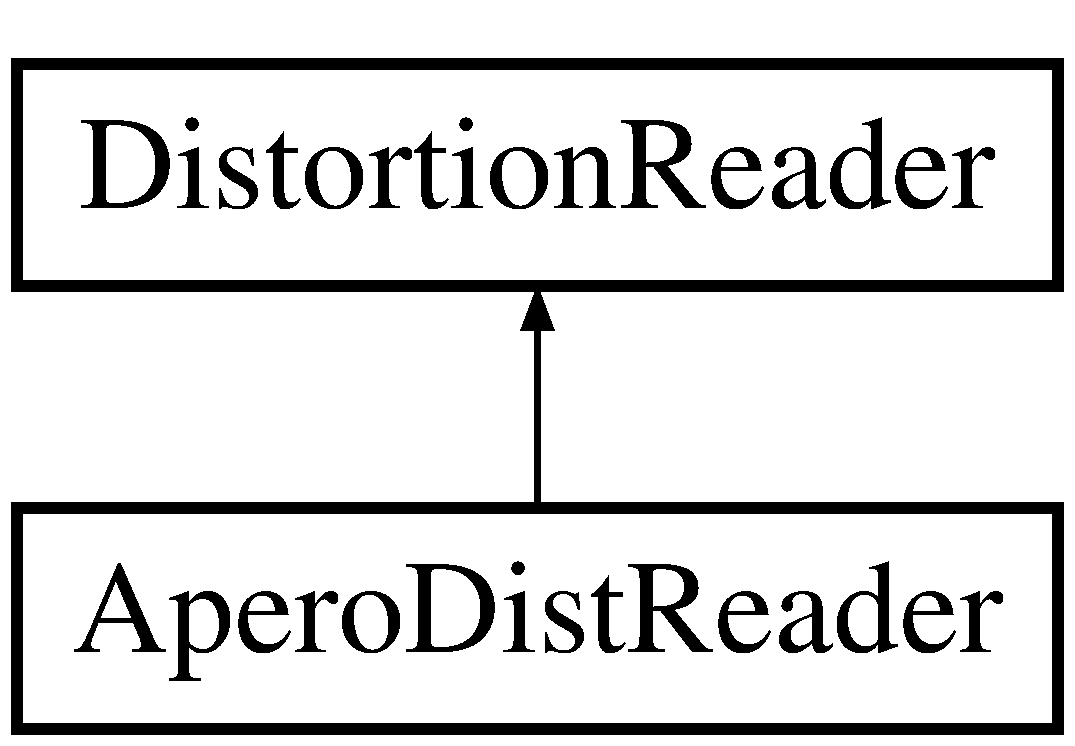
\includegraphics[height=2.000000cm]{classAperoDistReader}
\end{center}
\end{figure}
\subsection*{Public Member Functions}
\begin{DoxyCompactItemize}
\item 
\hypertarget{classAperoDistReader_a7646a9aef07ed08f35dc45bbf8dd25d5}{
\hyperlink{classAperoDistReader_a7646a9aef07ed08f35dc45bbf8dd25d5}{AperoDistReader} ()}
\label{classAperoDistReader_a7646a9aef07ed08f35dc45bbf8dd25d5}

\begin{DoxyCompactList}\small\item\em Constructor. \end{DoxyCompactList}\item 
virtual bool \hyperlink{classAperoDistReader_a363a91dd1581e99985cb298afbc9d16d}{read} (QIODevice $\ast$device)
\begin{DoxyCompactList}\small\item\em Reads a calibration file. \end{DoxyCompactList}\item 
virtual \hyperlink{classCamDistortion}{CamDistortion} $\ast$ \hyperlink{classAperoDistReader_a9a04faa9a3277270f51d1163965ce2ab}{getDistortion} ()
\begin{DoxyCompactList}\small\item\em Gets the camera distortion params, if it was read whith \char`\"{}read\char`\"{}. \end{DoxyCompactList}\end{DoxyCompactItemize}


\subsection{Detailed Description}
Reader for Apero camera calibration files whit Radial Distortion model. 

\subsection{Member Function Documentation}
\hypertarget{classAperoDistReader_a9a04faa9a3277270f51d1163965ce2ab}{
\index{AperoDistReader@{AperoDistReader}!getDistortion@{getDistortion}}
\index{getDistortion@{getDistortion}!AperoDistReader@{AperoDistReader}}
\subsubsection[{getDistortion}]{\setlength{\rightskip}{0pt plus 5cm}{\bf CamDistortion} $\ast$ AperoDistReader::getDistortion (
\begin{DoxyParamCaption}
{}
\end{DoxyParamCaption}
)\hspace{0.3cm}{\ttfamily  \mbox{[}virtual\mbox{]}}}}
\label{classAperoDistReader_a9a04faa9a3277270f51d1163965ce2ab}


Gets the camera distortion params, if it was read whith \char`\"{}read\char`\"{}. 

\begin{DoxyReturn}{Returns}
\hyperlink{classCamDistortion}{CamDistortion} $\ast$ camera distortion params 
\end{DoxyReturn}


Implements \hyperlink{classDistortionReader}{DistortionReader}.

\hypertarget{classAperoDistReader_a363a91dd1581e99985cb298afbc9d16d}{
\index{AperoDistReader@{AperoDistReader}!read@{read}}
\index{read@{read}!AperoDistReader@{AperoDistReader}}
\subsubsection[{read}]{\setlength{\rightskip}{0pt plus 5cm}bool AperoDistReader::read (
\begin{DoxyParamCaption}
\item[{QIODevice $\ast$}]{device}
\end{DoxyParamCaption}
)\hspace{0.3cm}{\ttfamily  \mbox{[}virtual\mbox{]}}}}
\label{classAperoDistReader_a363a91dd1581e99985cb298afbc9d16d}


Reads a calibration file. 


\begin{DoxyParams}{Parameters}
{\em device} & The input device (ie QFile $\ast$). \\
\hline
\end{DoxyParams}
\begin{DoxyReturn}{Returns}
bool True if device is a valid Apero calibration file (Radial Distortion Model). 
\end{DoxyReturn}


Implements \hyperlink{classDistortionReader}{DistortionReader}.



The documentation for this class was generated from the following files:\begin{DoxyCompactItemize}
\item 
AperoDistReader.h\item 
AperoDistReader.cpp\end{DoxyCompactItemize}

\hypertarget{classCamDistortion}{
\section{CamDistortion Class Reference}
\label{classCamDistortion}\index{CamDistortion@{CamDistortion}}
}


Base class representing camera distortion.  




{\ttfamily \#include $<$CamDistortion.h$>$}

Inheritance diagram for CamDistortion:\begin{figure}[H]
\begin{center}
\leavevmode
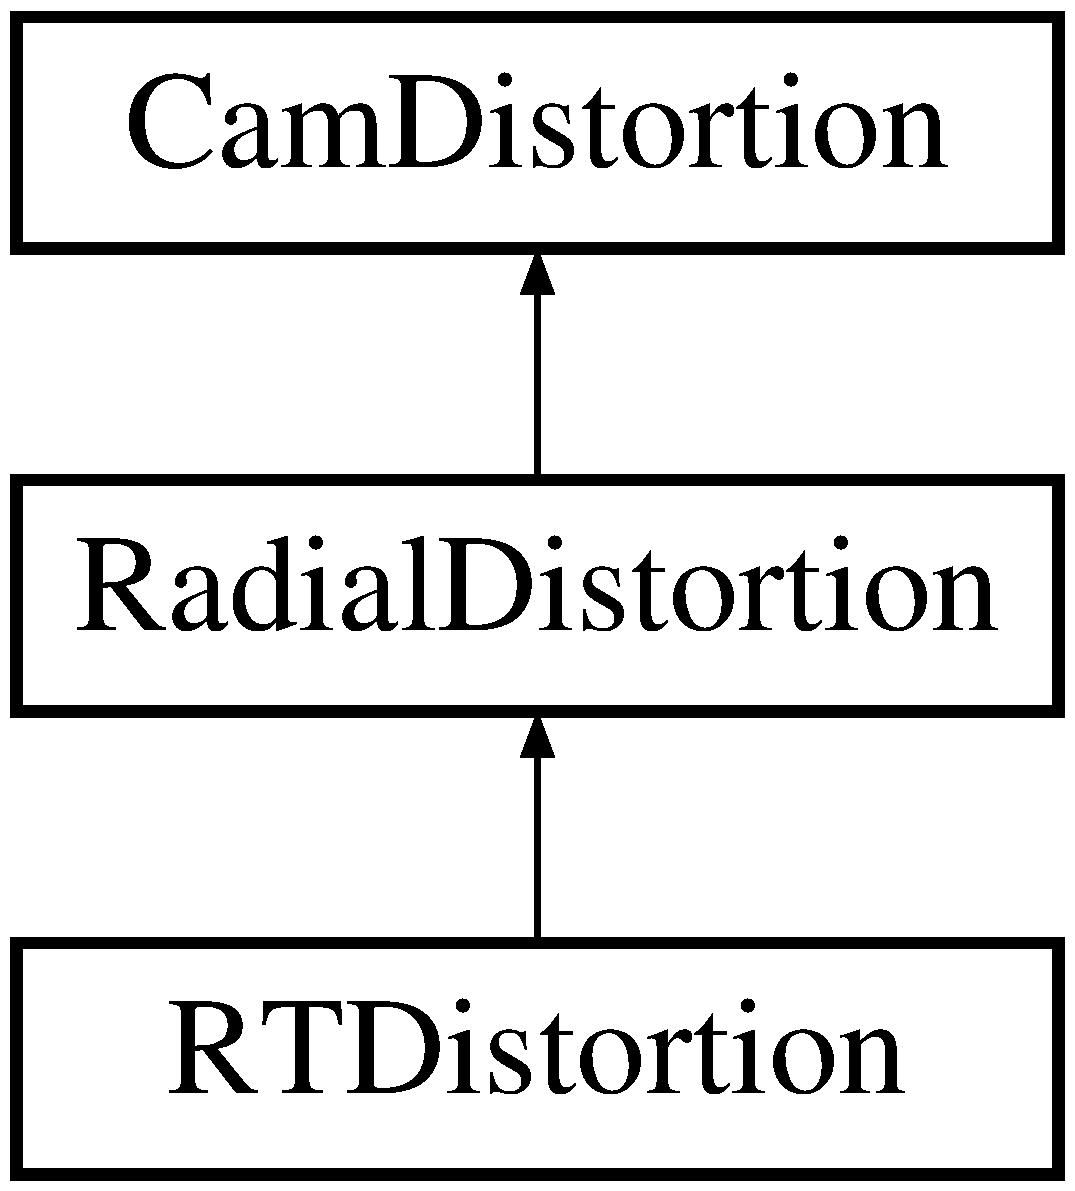
\includegraphics[height=3.000000cm]{classCamDistortion}
\end{center}
\end{figure}
\subsection*{Public Member Functions}
\begin{DoxyCompactItemize}
\item 
\hypertarget{classCamDistortion_afa8b5ea3910f856522246529911b0362}{
\hyperlink{classCamDistortion_afa8b5ea3910f856522246529911b0362}{CamDistortion} ()}
\label{classCamDistortion_afa8b5ea3910f856522246529911b0362}

\begin{DoxyCompactList}\small\item\em Contructor. \end{DoxyCompactList}\end{DoxyCompactItemize}


\subsection{Detailed Description}
Base class representing camera distortion. 

The documentation for this class was generated from the following files:\begin{DoxyCompactItemize}
\item 
CamDistortion.h\item 
CamDistortion.cpp\end{DoxyCompactItemize}

\hypertarget{classCameraModel}{
\section{CameraModel Class Reference}
\label{classCameraModel}\index{CameraModel@{CameraModel}}
}


Base class representing camera model.  




{\ttfamily \#include $<$CameraModel.h$>$}

Inheritance diagram for CameraModel:\begin{figure}[H]
\begin{center}
\leavevmode
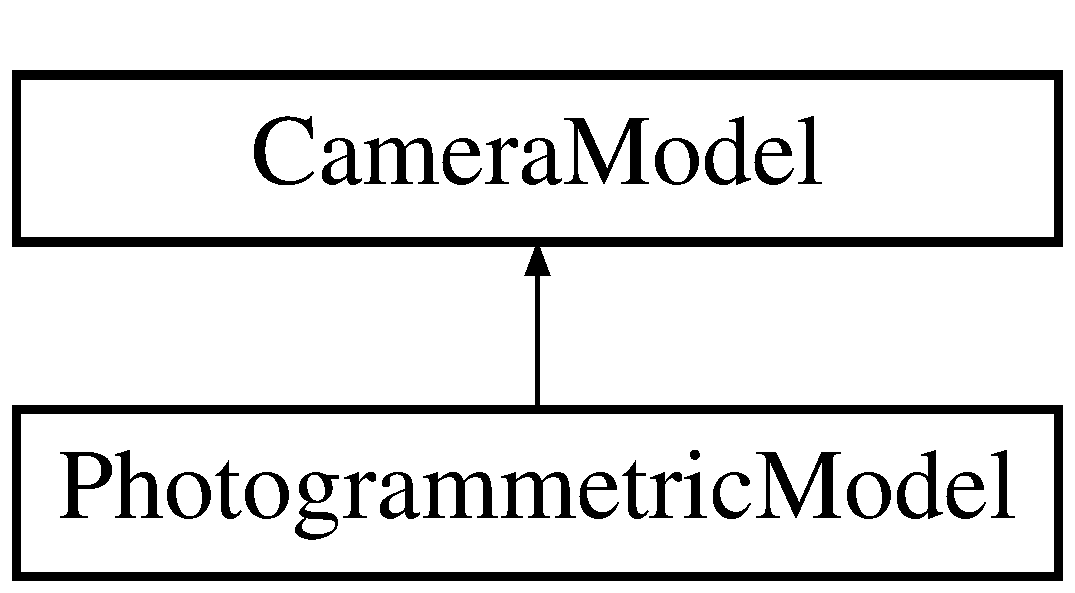
\includegraphics[height=2.000000cm]{classCameraModel}
\end{center}
\end{figure}
\subsection*{Public Member Functions}
\begin{DoxyCompactItemize}
\item 
\hypertarget{classCameraModel_a5d25add9bbcef6aaad94c26c1f28d418}{
\hyperlink{classCameraModel_a5d25add9bbcef6aaad94c26c1f28d418}{CameraModel} ()}
\label{classCameraModel_a5d25add9bbcef6aaad94c26c1f28d418}

\begin{DoxyCompactList}\small\item\em Constructor. \end{DoxyCompactList}\end{DoxyCompactItemize}


\subsection{Detailed Description}
Base class representing camera model. 

The documentation for this class was generated from the following files:\begin{DoxyCompactItemize}
\item 
CameraModel.h\item 
CameraModel.cpp\end{DoxyCompactItemize}

\hypertarget{classDecentering}{
\section{Decentering Class Reference}
\label{classDecentering}\index{Decentering@{Decentering}}
}
Inheritance diagram for Decentering:\begin{figure}[H]
\begin{center}
\leavevmode
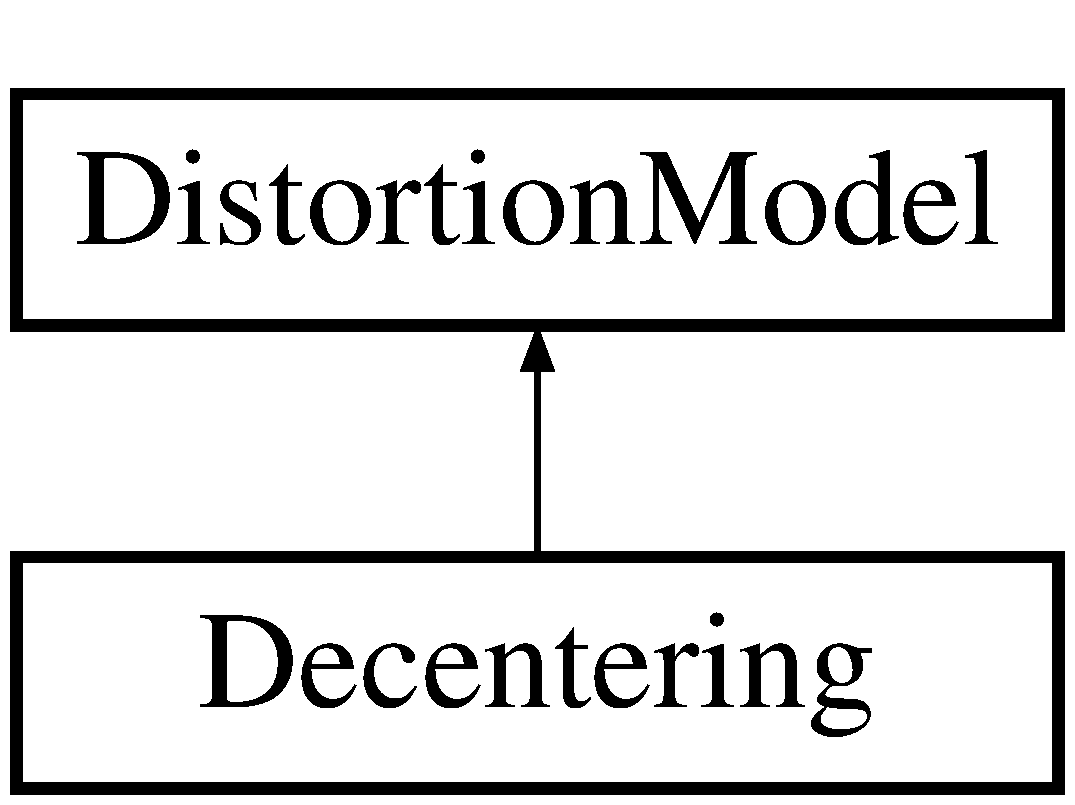
\includegraphics[height=2.000000cm]{classDecentering}
\end{center}
\end{figure}


The documentation for this class was generated from the following files:\begin{DoxyCompactItemize}
\item 
Decentering.h\item 
Decentering.cpp\end{DoxyCompactItemize}

\hypertarget{classDistortionModel}{
\section{DistortionModel Class Reference}
\label{classDistortionModel}\index{DistortionModel@{DistortionModel}}
}


Base class representing camera distortion model.  




{\ttfamily \#include $<$DistortionModel.h$>$}

Inheritance diagram for DistortionModel:\begin{figure}[H]
\begin{center}
\leavevmode
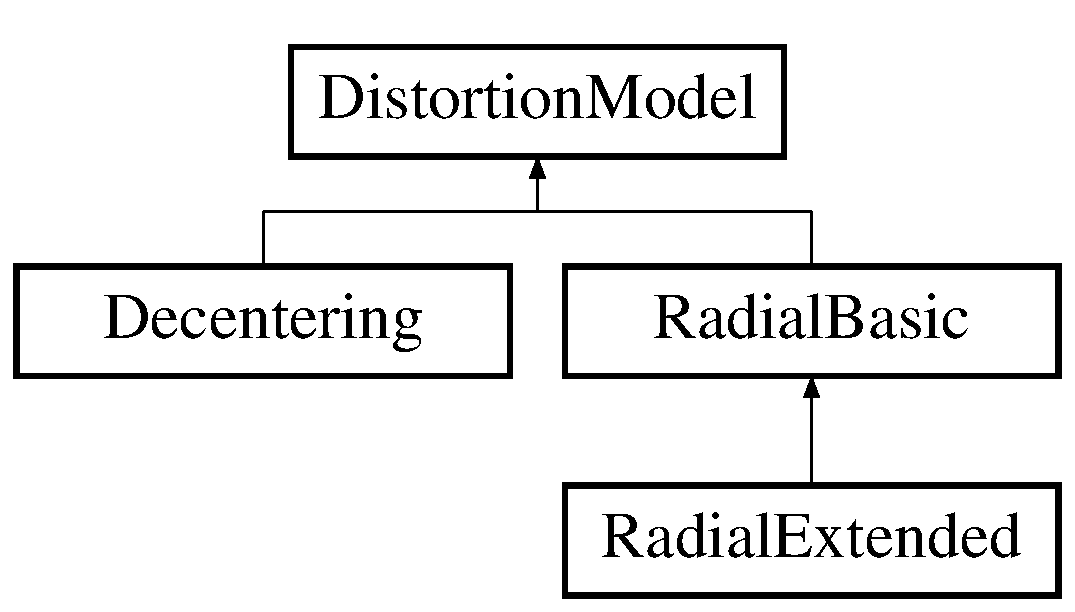
\includegraphics[height=3.000000cm]{classDistortionModel}
\end{center}
\end{figure}
\subsection*{Public Member Functions}
\begin{DoxyCompactItemize}
\item 
\hypertarget{classDistortionModel_a7d3ce5dc270e180b7b0594f2292b57d8}{
\hyperlink{classDistortionModel_a7d3ce5dc270e180b7b0594f2292b57d8}{DistortionModel} ()}
\label{classDistortionModel_a7d3ce5dc270e180b7b0594f2292b57d8}

\begin{DoxyCompactList}\small\item\em Constructor. \end{DoxyCompactList}\end{DoxyCompactItemize}


\subsection{Detailed Description}
Base class representing camera distortion model. 

The documentation for this class was generated from the following files:\begin{DoxyCompactItemize}
\item 
DistortionModel.h\item 
DistortionModel.cpp\end{DoxyCompactItemize}

\hypertarget{classDistortionReader}{
\section{DistortionReader Class Reference}
\label{classDistortionReader}\index{DistortionReader@{DistortionReader}}
}
Inheritance diagram for DistortionReader:\begin{figure}[H]
\begin{center}
\leavevmode
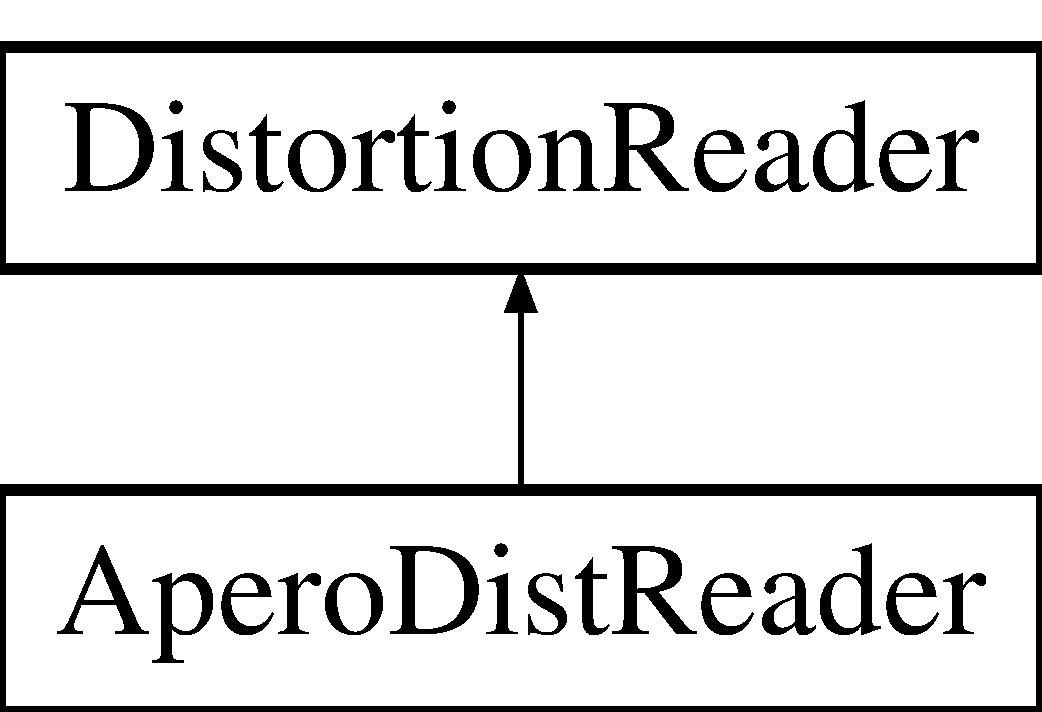
\includegraphics[height=2.000000cm]{classDistortionReader}
\end{center}
\end{figure}
\subsection*{Public Member Functions}
\begin{DoxyCompactItemize}
\item 
\hypertarget{classDistortionReader_a217d2c34193ad9ce256fed0b376a0b45}{
virtual bool {\bfseries read} (QIODevice $\ast$device)=0}
\label{classDistortionReader_a217d2c34193ad9ce256fed0b376a0b45}

\item 
\hypertarget{classDistortionReader_aafcd94d9f639e660049f1d9696570d8f}{
virtual \hyperlink{classCamDistortion}{CamDistortion} $\ast$ {\bfseries getDistortion} ()=0}
\label{classDistortionReader_aafcd94d9f639e660049f1d9696570d8f}

\end{DoxyCompactItemize}
\subsection*{Protected Attributes}
\begin{DoxyCompactItemize}
\item 
\hypertarget{classDistortionReader_a69facac6b79b5edb83e4c2f31409fd5f}{
\hyperlink{classCamDistortion}{CamDistortion} $\ast$ {\bfseries mCamDistortion}}
\label{classDistortionReader_a69facac6b79b5edb83e4c2f31409fd5f}

\end{DoxyCompactItemize}


The documentation for this class was generated from the following files:\begin{DoxyCompactItemize}
\item 
DistortionReader.h\item 
DistortionReader.cpp\end{DoxyCompactItemize}

\hypertarget{classLibPW}{
\section{LibPW Class Reference}
\label{classLibPW}\index{LibPW@{LibPW}}
}


The documentation for this class was generated from the following files:\begin{DoxyCompactItemize}
\item 
libPW.h\item 
libPW.cpp\end{DoxyCompactItemize}

\hypertarget{classPhotogrammetricModel}{
\section{PhotogrammetricModel Class Reference}
\label{classPhotogrammetricModel}\index{PhotogrammetricModel@{PhotogrammetricModel}}
}
Inheritance diagram for PhotogrammetricModel:\begin{figure}[H]
\begin{center}
\leavevmode
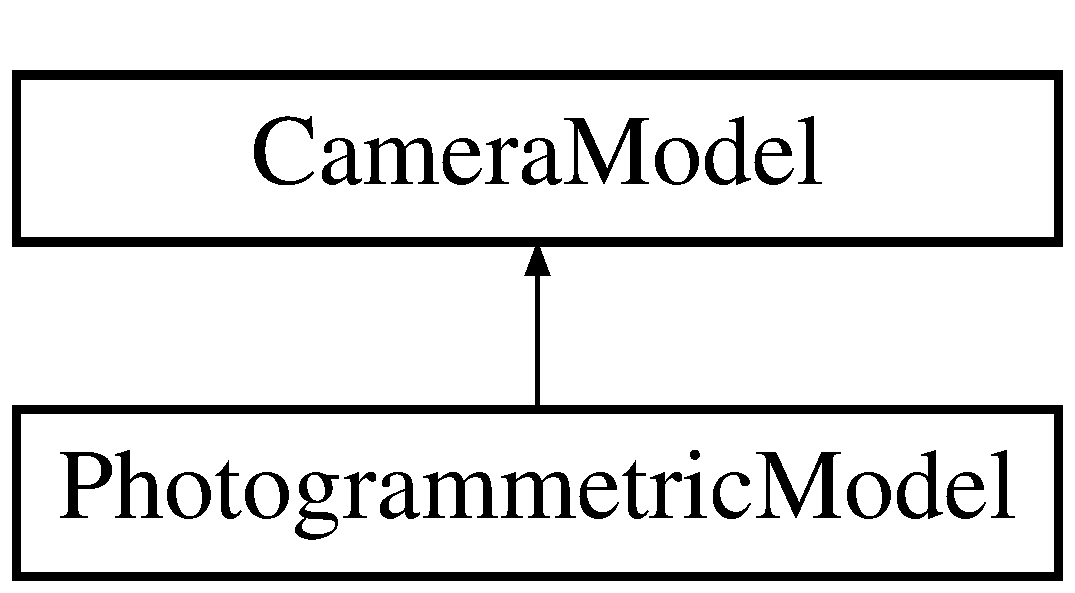
\includegraphics[height=2.000000cm]{classPhotogrammetricModel}
\end{center}
\end{figure}
\subsection*{Public Member Functions}
\begin{DoxyCompactItemize}
\item 
float \hyperlink{classPhotogrammetricModel_a8a801665a82d877695a61d4cf5452028}{getFocal} ()
\item 
float \hyperlink{classPhotogrammetricModel_a7768332a2d384718ced8023b91be32e1}{getXp} ()
\item 
float \hyperlink{classPhotogrammetricModel_af8281efc191b2fe5a2e81e7d4782314d}{getYp} ()
\item 
\hyperlink{classDistortionModel}{DistortionModel} $\ast$ \hyperlink{classPhotogrammetricModel_aeb0e1fa05c2f512c50306190a0ebf1b3}{getDistortionModel} ()
\item 
void \hyperlink{classPhotogrammetricModel_ab8fa3b15befb2615d93762eb41989048}{setFocal} (float f)
\item 
void \hyperlink{classPhotogrammetricModel_a33de1961133f9f61da8de26214f962df}{setXp} (float xp)
\item 
void \hyperlink{classPhotogrammetricModel_ae8c8671d1c891d51df97b223380b483d}{setYp} (float yp)
\item 
void \hyperlink{classPhotogrammetricModel_a5709d669a85998ae9b51d2b41de40dec}{setDistortionModel} (\hyperlink{classDistortionModel}{DistortionModel} $\ast$model)
\end{DoxyCompactItemize}


\subsection{Member Function Documentation}
\hypertarget{classPhotogrammetricModel_aeb0e1fa05c2f512c50306190a0ebf1b3}{
\index{PhotogrammetricModel@{PhotogrammetricModel}!getDistortionModel@{getDistortionModel}}
\index{getDistortionModel@{getDistortionModel}!PhotogrammetricModel@{PhotogrammetricModel}}
\subsubsection[{getDistortionModel}]{\setlength{\rightskip}{0pt plus 5cm}{\bf DistortionModel} $\ast$ PhotogrammetricModel::getDistortionModel (
\begin{DoxyParamCaption}
{}
\end{DoxyParamCaption}
)}}
\label{classPhotogrammetricModel_aeb0e1fa05c2f512c50306190a0ebf1b3}
\begin{DoxyReturn}{Returns}
\hyperlink{classDistortionModel}{DistortionModel} $\ast$ 
\end{DoxyReturn}
\hypertarget{classPhotogrammetricModel_a8a801665a82d877695a61d4cf5452028}{
\index{PhotogrammetricModel@{PhotogrammetricModel}!getFocal@{getFocal}}
\index{getFocal@{getFocal}!PhotogrammetricModel@{PhotogrammetricModel}}
\subsubsection[{getFocal}]{\setlength{\rightskip}{0pt plus 5cm}float PhotogrammetricModel::getFocal (
\begin{DoxyParamCaption}
{}
\end{DoxyParamCaption}
)}}
\label{classPhotogrammetricModel_a8a801665a82d877695a61d4cf5452028}
\begin{DoxyReturn}{Returns}
float 
\end{DoxyReturn}
\hypertarget{classPhotogrammetricModel_a7768332a2d384718ced8023b91be32e1}{
\index{PhotogrammetricModel@{PhotogrammetricModel}!getXp@{getXp}}
\index{getXp@{getXp}!PhotogrammetricModel@{PhotogrammetricModel}}
\subsubsection[{getXp}]{\setlength{\rightskip}{0pt plus 5cm}float PhotogrammetricModel::getXp (
\begin{DoxyParamCaption}
{}
\end{DoxyParamCaption}
)}}
\label{classPhotogrammetricModel_a7768332a2d384718ced8023b91be32e1}
\begin{DoxyReturn}{Returns}
float 
\end{DoxyReturn}
\hypertarget{classPhotogrammetricModel_af8281efc191b2fe5a2e81e7d4782314d}{
\index{PhotogrammetricModel@{PhotogrammetricModel}!getYp@{getYp}}
\index{getYp@{getYp}!PhotogrammetricModel@{PhotogrammetricModel}}
\subsubsection[{getYp}]{\setlength{\rightskip}{0pt plus 5cm}float PhotogrammetricModel::getYp (
\begin{DoxyParamCaption}
{}
\end{DoxyParamCaption}
)}}
\label{classPhotogrammetricModel_af8281efc191b2fe5a2e81e7d4782314d}
\begin{DoxyReturn}{Returns}
float 
\end{DoxyReturn}
\hypertarget{classPhotogrammetricModel_a5709d669a85998ae9b51d2b41de40dec}{
\index{PhotogrammetricModel@{PhotogrammetricModel}!setDistortionModel@{setDistortionModel}}
\index{setDistortionModel@{setDistortionModel}!PhotogrammetricModel@{PhotogrammetricModel}}
\subsubsection[{setDistortionModel}]{\setlength{\rightskip}{0pt plus 5cm}void PhotogrammetricModel::setDistortionModel (
\begin{DoxyParamCaption}
\item[{{\bf DistortionModel} $\ast$}]{model}
\end{DoxyParamCaption}
)}}
\label{classPhotogrammetricModel_a5709d669a85998ae9b51d2b41de40dec}

\begin{DoxyParams}{Parameters}
{\em model} & \\
\hline
\end{DoxyParams}
\hypertarget{classPhotogrammetricModel_ab8fa3b15befb2615d93762eb41989048}{
\index{PhotogrammetricModel@{PhotogrammetricModel}!setFocal@{setFocal}}
\index{setFocal@{setFocal}!PhotogrammetricModel@{PhotogrammetricModel}}
\subsubsection[{setFocal}]{\setlength{\rightskip}{0pt plus 5cm}void PhotogrammetricModel::setFocal (
\begin{DoxyParamCaption}
\item[{float}]{f}
\end{DoxyParamCaption}
)}}
\label{classPhotogrammetricModel_ab8fa3b15befb2615d93762eb41989048}

\begin{DoxyParams}{Parameters}
{\em f} & \\
\hline
\end{DoxyParams}
\hypertarget{classPhotogrammetricModel_a33de1961133f9f61da8de26214f962df}{
\index{PhotogrammetricModel@{PhotogrammetricModel}!setXp@{setXp}}
\index{setXp@{setXp}!PhotogrammetricModel@{PhotogrammetricModel}}
\subsubsection[{setXp}]{\setlength{\rightskip}{0pt plus 5cm}void PhotogrammetricModel::setXp (
\begin{DoxyParamCaption}
\item[{float}]{xp}
\end{DoxyParamCaption}
)}}
\label{classPhotogrammetricModel_a33de1961133f9f61da8de26214f962df}

\begin{DoxyParams}{Parameters}
{\em xp} & \\
\hline
\end{DoxyParams}
\hypertarget{classPhotogrammetricModel_ae8c8671d1c891d51df97b223380b483d}{
\index{PhotogrammetricModel@{PhotogrammetricModel}!setYp@{setYp}}
\index{setYp@{setYp}!PhotogrammetricModel@{PhotogrammetricModel}}
\subsubsection[{setYp}]{\setlength{\rightskip}{0pt plus 5cm}void PhotogrammetricModel::setYp (
\begin{DoxyParamCaption}
\item[{float}]{yp}
\end{DoxyParamCaption}
)}}
\label{classPhotogrammetricModel_ae8c8671d1c891d51df97b223380b483d}

\begin{DoxyParams}{Parameters}
{\em yp} & \\
\hline
\end{DoxyParams}


The documentation for this class was generated from the following files:\begin{DoxyCompactItemize}
\item 
PhotogrammetricModel.h\item 
PhotogrammetricModel.cpp\end{DoxyCompactItemize}

\hypertarget{classRadialBasic}{
\section{RadialBasic Class Reference}
\label{classRadialBasic}\index{RadialBasic@{RadialBasic}}
}
Inheritance diagram for RadialBasic:\begin{figure}[H]
\begin{center}
\leavevmode
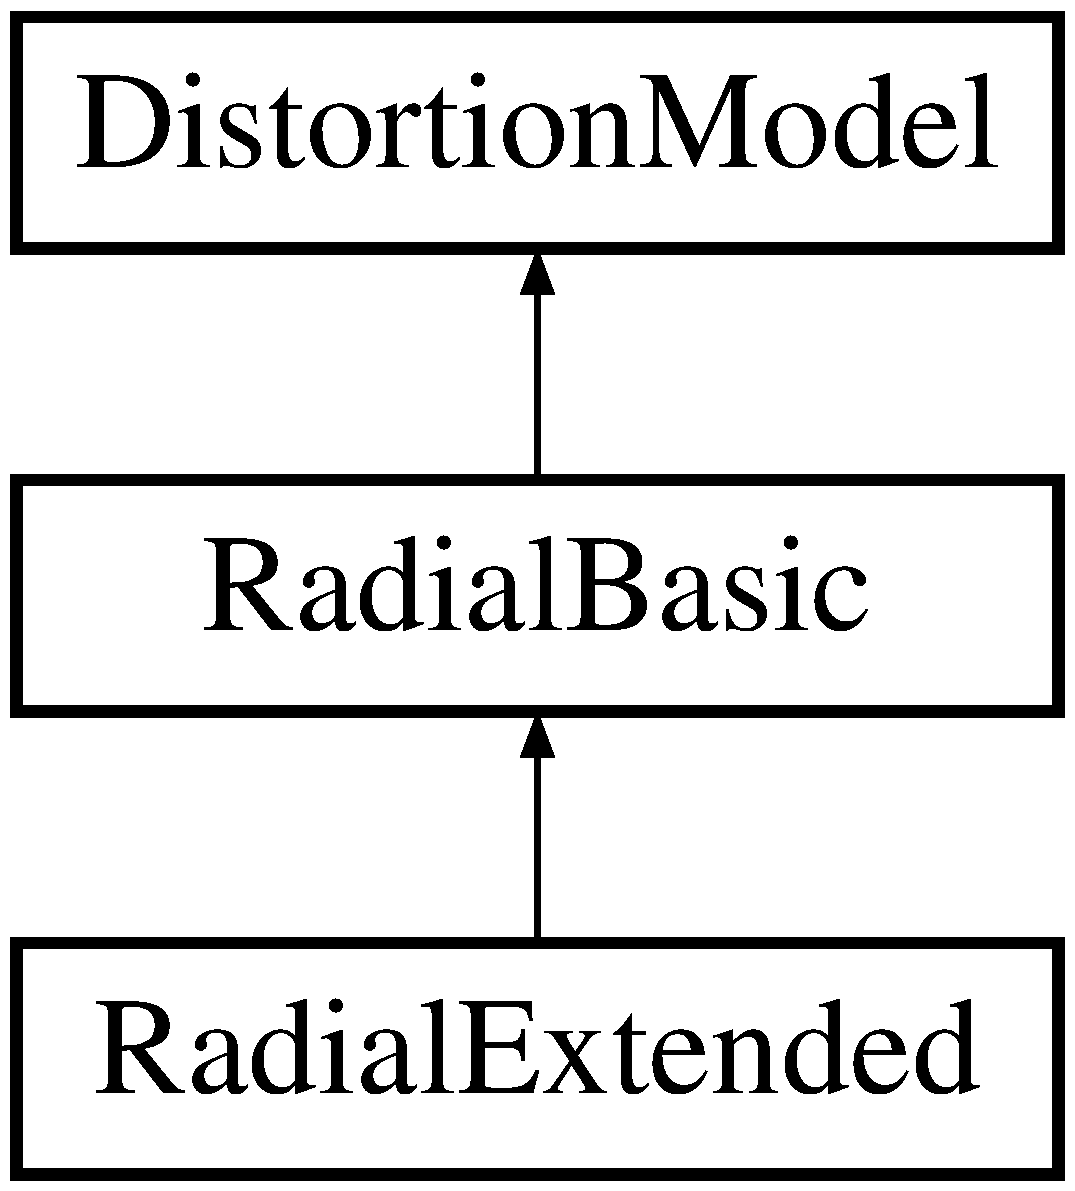
\includegraphics[height=3.000000cm]{classRadialBasic}
\end{center}
\end{figure}


The documentation for this class was generated from the following files:\begin{DoxyCompactItemize}
\item 
RadialBasic.h\item 
RadialBasic.cpp\end{DoxyCompactItemize}

\hypertarget{classRadialDistortion}{
\section{RadialDistortion Class Reference}
\label{classRadialDistortion}\index{RadialDistortion@{RadialDistortion}}
}


Base class representing camera distortion as radial distortion model.  




{\ttfamily \#include $<$RadialDistortion.h$>$}

Inheritance diagram for RadialDistortion:\begin{figure}[H]
\begin{center}
\leavevmode
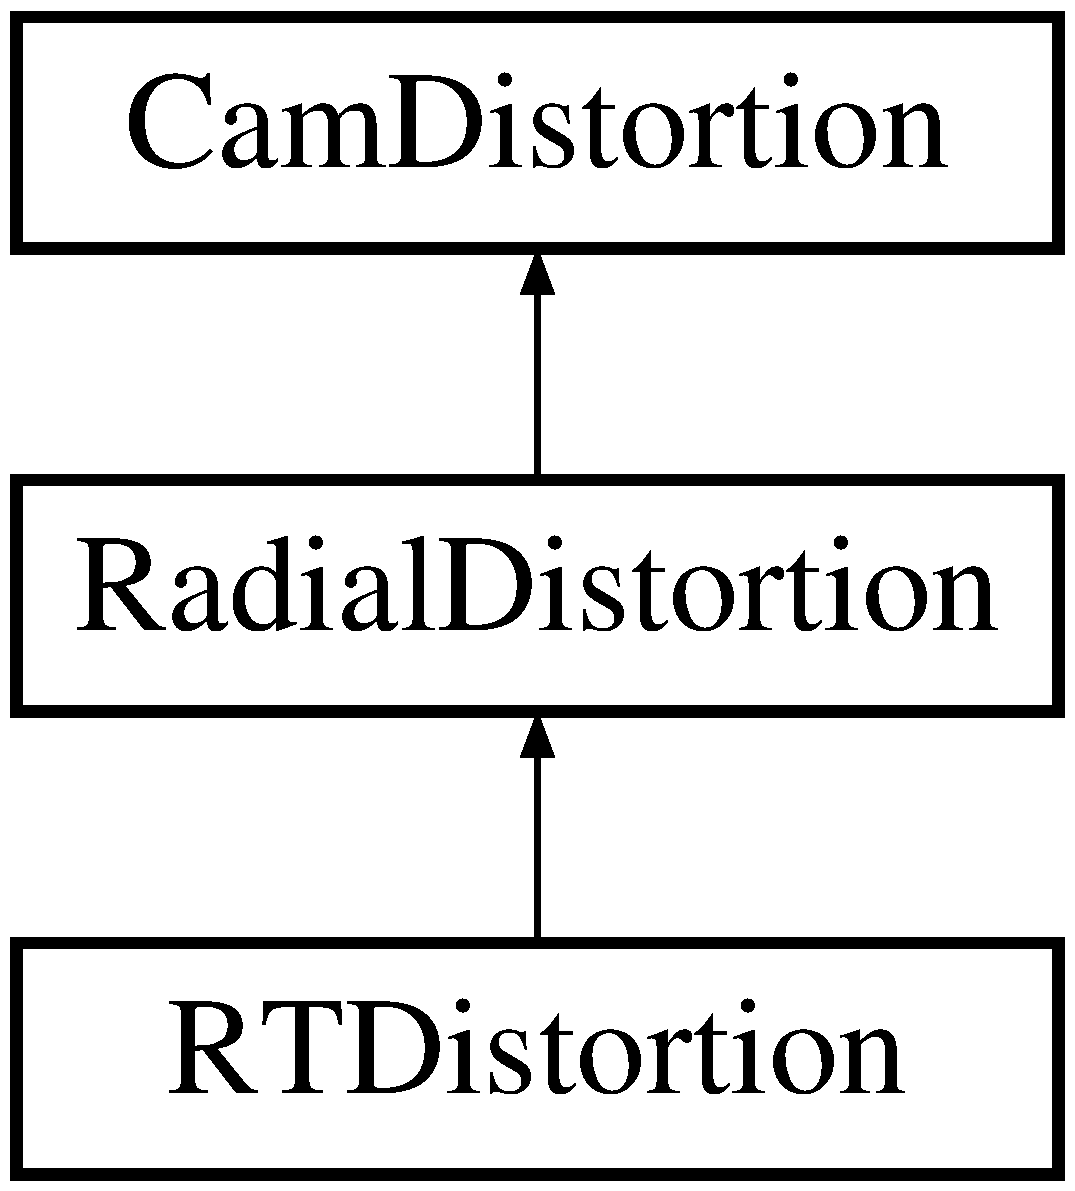
\includegraphics[height=3.000000cm]{classRadialDistortion}
\end{center}
\end{figure}
\subsection*{Public Member Functions}
\begin{DoxyCompactItemize}
\item 
\hypertarget{classRadialDistortion_a826307c3d60aa4756ec9adf460073782}{
\hyperlink{classRadialDistortion_a826307c3d60aa4756ec9adf460073782}{RadialDistortion} ()}
\label{classRadialDistortion_a826307c3d60aa4756ec9adf460073782}

\begin{DoxyCompactList}\small\item\em Constructor. \end{DoxyCompactList}\item 
\hypertarget{classRadialDistortion_ac19043a2dc84d988bca338c423e3f4e3}{
\hyperlink{classRadialDistortion_ac19043a2dc84d988bca338c423e3f4e3}{$\sim$RadialDistortion} ()}
\label{classRadialDistortion_ac19043a2dc84d988bca338c423e3f4e3}

\begin{DoxyCompactList}\small\item\em Destructor. \end{DoxyCompactList}\item 
float \hyperlink{classRadialDistortion_afa274c5fc6b2572a43f6b089f36c95a3}{getPP} ()
\begin{DoxyCompactList}\small\item\em Gets the principal ponit value in pixels. \end{DoxyCompactList}\item 
float \hyperlink{classRadialDistortion_aac0908909ad5c3f56fafcddc31999866}{getSymmetryPP} ()
\begin{DoxyCompactList}\small\item\em Gets the principal poin of symmetry in pixels. \end{DoxyCompactList}\item 
float \hyperlink{classRadialDistortion_ae51e183f957c6269a978eb46b6a69e5c}{getFocal} ()
\begin{DoxyCompactList}\small\item\em Gets the focal lenght in pixels. \end{DoxyCompactList}\item 
float \hyperlink{classRadialDistortion_ae10fc8e7de7476496e215c57bf90387e}{getRadialDistCoef} (int index)
\begin{DoxyCompactList}\small\item\em Gets a coefficient of radial distortion. \end{DoxyCompactList}\item 
int \hyperlink{classRadialDistortion_a6614a583264fc377d399ae387729b8cf}{getImageHeight} ()
\begin{DoxyCompactList}\small\item\em Gets the image height in pixels. \end{DoxyCompactList}\item 
int \hyperlink{classRadialDistortion_ae5bdbbef396660ea4e140c805390b36c}{getImageWidt} ()
\begin{DoxyCompactList}\small\item\em gets the image widt in pixels. \end{DoxyCompactList}\item 
void \hyperlink{classRadialDistortion_a9907642ef2898cda781084b1daead3c7}{setPP} (float pp)
\begin{DoxyCompactList}\small\item\em Sets the principal ponit value in pixels. \end{DoxyCompactList}\item 
void \hyperlink{classRadialDistortion_a91d59c0c97e7660604089cbb2e0cc743}{setSymmetryPP} (float symmetryPP)
\begin{DoxyCompactList}\small\item\em Sets the principal poin of symmetry in pixels. \end{DoxyCompactList}\item 
void \hyperlink{classRadialDistortion_a6418c0ee8375e4d6056ae44ebf30df19}{setFocal} (float f)
\begin{DoxyCompactList}\small\item\em Sets the focal lenght in pixels. \end{DoxyCompactList}\item 
void \hyperlink{classRadialDistortion_ace02ac046e219192c2b43ff2f7121da4}{setImageHeight} (int height)
\begin{DoxyCompactList}\small\item\em Sets the image height in pixels. \end{DoxyCompactList}\item 
void \hyperlink{classRadialDistortion_a468ca185db05d2026af41f771a28992b}{setImageWidt} (int widt)
\begin{DoxyCompactList}\small\item\em Sets the image widt in pixels. \end{DoxyCompactList}\item 
void \hyperlink{classRadialDistortion_ae1a625f4c64b14565b614ab676054a47}{addRadialCoef} (float coef)
\begin{DoxyCompactList}\small\item\em Append a coefficient of radial distortion at the of the coefficients vector. \end{DoxyCompactList}\end{DoxyCompactItemize}


\subsection{Detailed Description}
Base class representing camera distortion as radial distortion model. 

\subsection{Member Function Documentation}
\hypertarget{classRadialDistortion_ae1a625f4c64b14565b614ab676054a47}{
\index{RadialDistortion@{RadialDistortion}!addRadialCoef@{addRadialCoef}}
\index{addRadialCoef@{addRadialCoef}!RadialDistortion@{RadialDistortion}}
\subsubsection[{addRadialCoef}]{\setlength{\rightskip}{0pt plus 5cm}void RadialDistortion::addRadialCoef (
\begin{DoxyParamCaption}
\item[{float}]{coef}
\end{DoxyParamCaption}
)}}
\label{classRadialDistortion_ae1a625f4c64b14565b614ab676054a47}


Append a coefficient of radial distortion at the of the coefficients vector. 


\begin{DoxyParams}{Parameters}
{\em coef} & A coefficient of radial distortion. \\
\hline
\end{DoxyParams}
\hypertarget{classRadialDistortion_ae51e183f957c6269a978eb46b6a69e5c}{
\index{RadialDistortion@{RadialDistortion}!getFocal@{getFocal}}
\index{getFocal@{getFocal}!RadialDistortion@{RadialDistortion}}
\subsubsection[{getFocal}]{\setlength{\rightskip}{0pt plus 5cm}float RadialDistortion::getFocal (
\begin{DoxyParamCaption}
{}
\end{DoxyParamCaption}
)}}
\label{classRadialDistortion_ae51e183f957c6269a978eb46b6a69e5c}


Gets the focal lenght in pixels. 

\begin{DoxyReturn}{Returns}
float focal lenght in pixels. 
\end{DoxyReturn}
\hypertarget{classRadialDistortion_a6614a583264fc377d399ae387729b8cf}{
\index{RadialDistortion@{RadialDistortion}!getImageHeight@{getImageHeight}}
\index{getImageHeight@{getImageHeight}!RadialDistortion@{RadialDistortion}}
\subsubsection[{getImageHeight}]{\setlength{\rightskip}{0pt plus 5cm}int RadialDistortion::getImageHeight (
\begin{DoxyParamCaption}
{}
\end{DoxyParamCaption}
)}}
\label{classRadialDistortion_a6614a583264fc377d399ae387729b8cf}


Gets the image height in pixels. 

\begin{DoxyReturn}{Returns}
int image height in pixels. 
\end{DoxyReturn}
\hypertarget{classRadialDistortion_ae5bdbbef396660ea4e140c805390b36c}{
\index{RadialDistortion@{RadialDistortion}!getImageWidt@{getImageWidt}}
\index{getImageWidt@{getImageWidt}!RadialDistortion@{RadialDistortion}}
\subsubsection[{getImageWidt}]{\setlength{\rightskip}{0pt plus 5cm}int RadialDistortion::getImageWidt (
\begin{DoxyParamCaption}
{}
\end{DoxyParamCaption}
)}}
\label{classRadialDistortion_ae5bdbbef396660ea4e140c805390b36c}


gets the image widt in pixels. 

\begin{DoxyReturn}{Returns}
int Image widt in pixels. 
\end{DoxyReturn}
\hypertarget{classRadialDistortion_afa274c5fc6b2572a43f6b089f36c95a3}{
\index{RadialDistortion@{RadialDistortion}!getPP@{getPP}}
\index{getPP@{getPP}!RadialDistortion@{RadialDistortion}}
\subsubsection[{getPP}]{\setlength{\rightskip}{0pt plus 5cm}float RadialDistortion::getPP (
\begin{DoxyParamCaption}
{}
\end{DoxyParamCaption}
)}}
\label{classRadialDistortion_afa274c5fc6b2572a43f6b089f36c95a3}


Gets the principal ponit value in pixels. 

\begin{DoxyReturn}{Returns}
float principal point in pixels. 
\end{DoxyReturn}
\hypertarget{classRadialDistortion_ae10fc8e7de7476496e215c57bf90387e}{
\index{RadialDistortion@{RadialDistortion}!getRadialDistCoef@{getRadialDistCoef}}
\index{getRadialDistCoef@{getRadialDistCoef}!RadialDistortion@{RadialDistortion}}
\subsubsection[{getRadialDistCoef}]{\setlength{\rightskip}{0pt plus 5cm}float RadialDistortion::getRadialDistCoef (
\begin{DoxyParamCaption}
\item[{int}]{index}
\end{DoxyParamCaption}
)}}
\label{classRadialDistortion_ae10fc8e7de7476496e215c57bf90387e}


Gets a coefficient of radial distortion. 


\begin{DoxyParams}{Parameters}
{\em index} & Position of the coefficient in the vector of coefficients. \\
\hline
\end{DoxyParams}
\begin{DoxyReturn}{Returns}
float the coefficient at position indicated by index. 
\end{DoxyReturn}
\hypertarget{classRadialDistortion_aac0908909ad5c3f56fafcddc31999866}{
\index{RadialDistortion@{RadialDistortion}!getSymmetryPP@{getSymmetryPP}}
\index{getSymmetryPP@{getSymmetryPP}!RadialDistortion@{RadialDistortion}}
\subsubsection[{getSymmetryPP}]{\setlength{\rightskip}{0pt plus 5cm}float RadialDistortion::getSymmetryPP (
\begin{DoxyParamCaption}
{}
\end{DoxyParamCaption}
)}}
\label{classRadialDistortion_aac0908909ad5c3f56fafcddc31999866}


Gets the principal poin of symmetry in pixels. 

\begin{DoxyReturn}{Returns}
float principal poin of symmetry in pixels. 
\end{DoxyReturn}
\hypertarget{classRadialDistortion_a6418c0ee8375e4d6056ae44ebf30df19}{
\index{RadialDistortion@{RadialDistortion}!setFocal@{setFocal}}
\index{setFocal@{setFocal}!RadialDistortion@{RadialDistortion}}
\subsubsection[{setFocal}]{\setlength{\rightskip}{0pt plus 5cm}void RadialDistortion::setFocal (
\begin{DoxyParamCaption}
\item[{float}]{f}
\end{DoxyParamCaption}
)}}
\label{classRadialDistortion_a6418c0ee8375e4d6056ae44ebf30df19}


Sets the focal lenght in pixels. 


\begin{DoxyParams}{Parameters}
{\em f} & focal lenght in pixels. \\
\hline
\end{DoxyParams}
\hypertarget{classRadialDistortion_ace02ac046e219192c2b43ff2f7121da4}{
\index{RadialDistortion@{RadialDistortion}!setImageHeight@{setImageHeight}}
\index{setImageHeight@{setImageHeight}!RadialDistortion@{RadialDistortion}}
\subsubsection[{setImageHeight}]{\setlength{\rightskip}{0pt plus 5cm}void RadialDistortion::setImageHeight (
\begin{DoxyParamCaption}
\item[{int}]{height}
\end{DoxyParamCaption}
)}}
\label{classRadialDistortion_ace02ac046e219192c2b43ff2f7121da4}


Sets the image height in pixels. 


\begin{DoxyParams}{Parameters}
{\em height} & the image height in pixels. \\
\hline
\end{DoxyParams}
\hypertarget{classRadialDistortion_a468ca185db05d2026af41f771a28992b}{
\index{RadialDistortion@{RadialDistortion}!setImageWidt@{setImageWidt}}
\index{setImageWidt@{setImageWidt}!RadialDistortion@{RadialDistortion}}
\subsubsection[{setImageWidt}]{\setlength{\rightskip}{0pt plus 5cm}void RadialDistortion::setImageWidt (
\begin{DoxyParamCaption}
\item[{int}]{widt}
\end{DoxyParamCaption}
)}}
\label{classRadialDistortion_a468ca185db05d2026af41f771a28992b}


Sets the image widt in pixels. 


\begin{DoxyParams}{Parameters}
{\em widt} & the image widt in pixels. \\
\hline
\end{DoxyParams}
\hypertarget{classRadialDistortion_a9907642ef2898cda781084b1daead3c7}{
\index{RadialDistortion@{RadialDistortion}!setPP@{setPP}}
\index{setPP@{setPP}!RadialDistortion@{RadialDistortion}}
\subsubsection[{setPP}]{\setlength{\rightskip}{0pt plus 5cm}void RadialDistortion::setPP (
\begin{DoxyParamCaption}
\item[{float}]{pp}
\end{DoxyParamCaption}
)}}
\label{classRadialDistortion_a9907642ef2898cda781084b1daead3c7}


Sets the principal ponit value in pixels. 


\begin{DoxyParams}{Parameters}
{\em pp} & principal ponit value in pixels. \\
\hline
\end{DoxyParams}
\hypertarget{classRadialDistortion_a91d59c0c97e7660604089cbb2e0cc743}{
\index{RadialDistortion@{RadialDistortion}!setSymmetryPP@{setSymmetryPP}}
\index{setSymmetryPP@{setSymmetryPP}!RadialDistortion@{RadialDistortion}}
\subsubsection[{setSymmetryPP}]{\setlength{\rightskip}{0pt plus 5cm}void RadialDistortion::setSymmetryPP (
\begin{DoxyParamCaption}
\item[{float}]{symmetryPP}
\end{DoxyParamCaption}
)}}
\label{classRadialDistortion_a91d59c0c97e7660604089cbb2e0cc743}


Sets the principal poin of symmetry in pixels. 


\begin{DoxyParams}{Parameters}
{\em symmetryPP} & principal poin of symmetry in pixels. \\
\hline
\end{DoxyParams}


The documentation for this class was generated from the following files:\begin{DoxyCompactItemize}
\item 
RadialDistortion.h\item 
RadialDistortion.cpp\end{DoxyCompactItemize}

\hypertarget{classRadialExtended}{
\section{RadialExtended Class Reference}
\label{classRadialExtended}\index{RadialExtended@{RadialExtended}}
}
Inheritance diagram for RadialExtended:\begin{figure}[H]
\begin{center}
\leavevmode
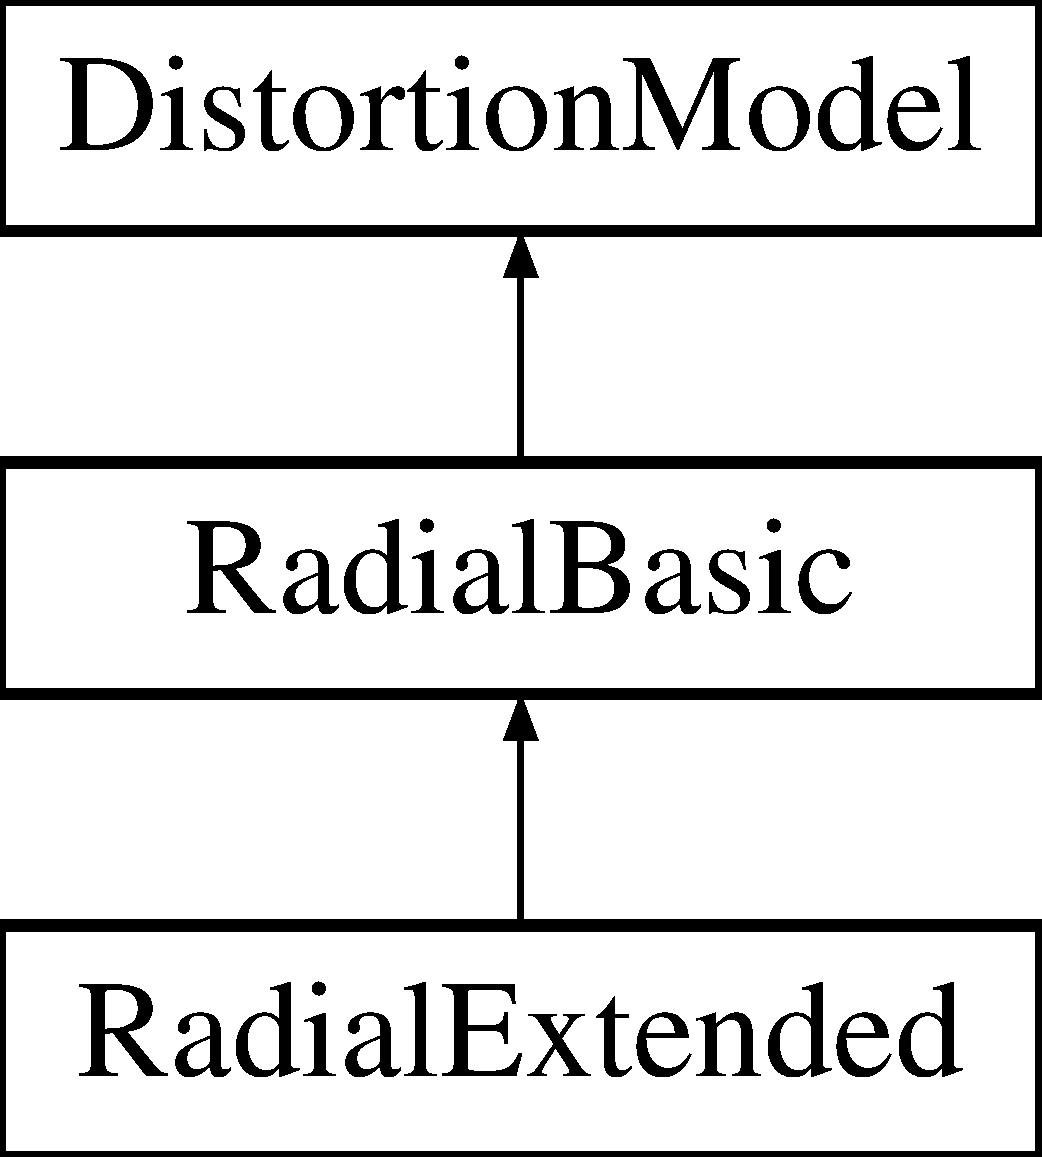
\includegraphics[height=3.000000cm]{classRadialExtended}
\end{center}
\end{figure}


The documentation for this class was generated from the following files:\begin{DoxyCompactItemize}
\item 
RadialExtended.h\item 
RadialExtended.cpp\end{DoxyCompactItemize}

\hypertarget{classRTDistortion}{
\section{RTDistortion Class Reference}
\label{classRTDistortion}\index{RTDistortion@{RTDistortion}}
}
Inheritance diagram for RTDistortion:\begin{figure}[H]
\begin{center}
\leavevmode
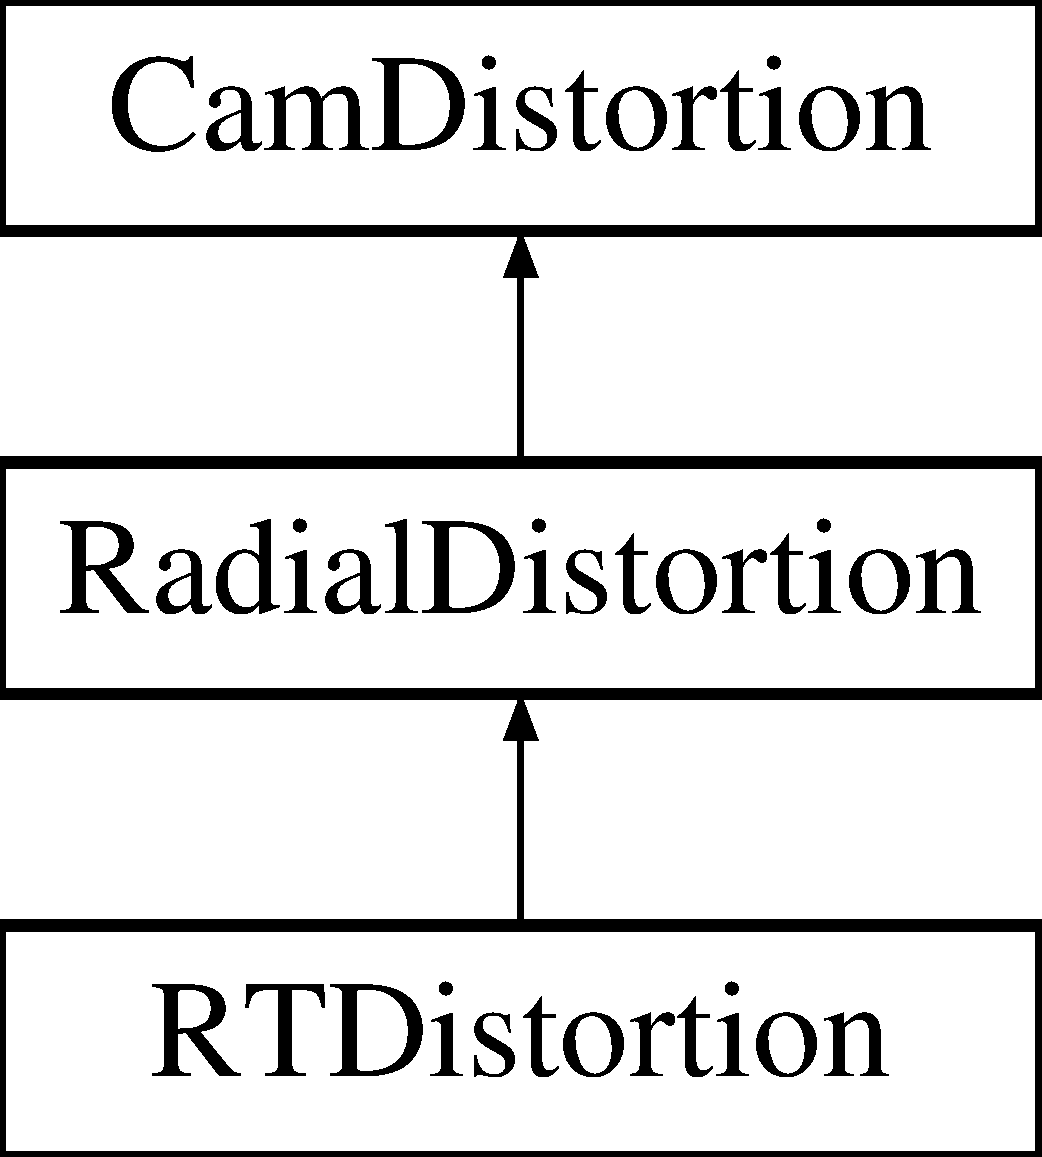
\includegraphics[height=3.000000cm]{classRTDistortion}
\end{center}
\end{figure}


The documentation for this class was generated from the following files:\begin{DoxyCompactItemize}
\item 
RTDistortion.h\item 
RTDistortion.cpp\end{DoxyCompactItemize}

\printindex
\end{document}
